%!TEX root = main.tex

\section{The Frank-Wolfe Method}\index{Frank-Wolfe method}\index{Conditional-Gradient method|see {Frank-Wolfe method}}

Also known as the \emph{Conditional-Gradient method}, it is widely used to solve programs where the feasibility region $S$ is described by a system of linear inequalities.
\begin{equation*}
(P): \begin{cases} \displaystyle{\min_{\x\in S}f(\x)} \\ S=\{ \x \in \field{R}^d:  \langle \boldsymbol{a}_k, \x \rangle \leq b_k \text{ with } \boldsymbol{a}_k \in \field{R}^d, b_k \in \field{R}, 1\leq k \leq \ell  \}
\end{cases}
\end{equation*}

This is an iterative method that, at any feasible initial guess $\x_0 \in S$, considers an associated linear program $(LP_0)$ that minimizes the linear approximation $L_0(\x) = f(\x_0) + \langle \gradient{f}(\x_0), \x - \x_0 \rangle$ on the same feasible region $S$.
\begin{equation*}
(LP_0): \begin{cases} \displaystyle{\min_{\x \in S} \langle \gradient{f}(\x_0), \x-\x_0 \rangle} \\
 S =\{ \x \in \field{R}^d:  \langle \boldsymbol{a}_k, \x \rangle \leq b_k \text{ with } \boldsymbol{a}_k \in \field{R}^d, b_k \in \field{R}, 1\leq k \leq \ell  \}
 \end{cases}
\end{equation*}
Once an optimal solution $\bar{\x}_0$ of $(LP_0)$ has been obtained, a line-search\index{Line-search} is performed on the segment joining $\x_0$ with $\bar{\x}_0$ (which by hypothesis is contained in the feasibility region $S$). 
\begin{equation*}
t_0 = \argmin_{0\leq t \leq 1} f\big(\x_0 + t(\bar{\x}_0-\x_0) \big).
\end{equation*}
Set then $x_1 = \x_0 + t_0 (\bar{\x}_0-\x_0)$.  We repeat this process to obtain a sequence $\{\x_n\}_{n\in\field{N}}$ of feasible points.

We usually devise a \emph{stopping criteria} (given a fixed tolerance $\varepsilon>0$) to guarantee that we are close enough to the optimal solution of $(P)$.  An example of such a process is illustrated below:\index{Frank-Wolfe method!stopping criteria}\index{Frank-Wolfe method!lower bound}\index{Frank-Wolfe method!upper bound}
\begin{description}
\item [Initialization] Let $\x_0 \in S$ be an initial feasible guess, and set $LB=-\infty$, $UB=f(\x_0)$---the \emph{lower} and \emph{upper} bounds (respectively) for the stopping criteria.
\item [Iteration] Assume we have $\x_n$, $LB$, $UB$.  Set 
\begin{equation*}
L_n(\x) = f(\x_n) + \langle \gradient{f}(\x_n), \x-\x_n \rangle. 
\end{equation*}
Find
\begin{align*}
\bar{\x}_n &= \argmin_{\x \in S} L_n(\x) = \argmin_{\x \in S} \langle \gradient{f}(\x_n), \x-\x_n \rangle,\\
\xi_n &= \min_{\x \in S} L_n(\x) = L_n(\bar{\x}_n),\\
t_n &= \argmin_{0 \leq t \leq 1} f\big(\x_n + t(\x_n - \bar{\x}_n)\big), \\
\x_{n+1} &= \x_n + t_n (\x_n - \bar{\x}_n), \\
LB &= \max(LB, \xi_n)
\end{align*}
\item [Stopping Criteria] If $\lvert UB-LB \rvert \leq \varepsilon$, then stop. Otherwise, update the upper bound, $UB = f(\x_{n+1})$, and perform the next \textbf{Iteration}.
\end{description}

\begin{example}\label{example:FrankWolfe}
Let us use this technique to try and find the minimum value of the function $f(x,y)=(x-3)^2+(y-2)^2$ over the square with vertices at $(-3/2, 0)$, $(0, 3/2)$, $(3/2, 0)$ and $(0, -3/2)$. We start by defining the inequality constraints:
\begin{align*}
g_1(x,y) &= x+y-\tfrac{3}{2} = \langle [1,1], [x,y] \rangle - \tfrac{3}{2} \\
g_2(x,y) &= x-y-\tfrac{3}{2} = \langle [1,-1], [x,y] \rangle - \tfrac{3}{2} \\
g_3(x,y) &= -x-y-\tfrac{3}{2} = \langle [-1,-1], [x,y] \rangle - \tfrac{3}{2} \\
g_4(x,y) &= -x+y-\tfrac{3}{2} = \langle [-1,1], [x,y] \rangle - \tfrac{3}{2}
\end{align*}
\begin{figure}[ht!]
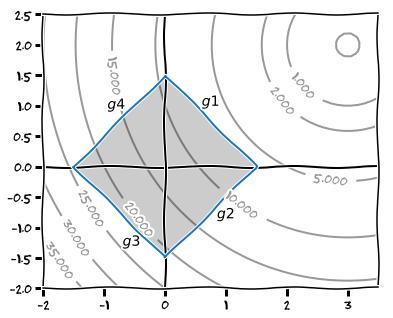
\includegraphics[width=0.75\linewidth]{Extras/frankwolfesetup.png}
\caption{Set up for example \ref{example:FrankWolfe}}\label{figure:FrankWolfesetup}
\end{figure}
We also need the gradient of $f$: $\gradient{f}(x,y) = \big[ 2(x-3), 2(y-2) \big]$. At any point $(x_0,y_0)$, the linear approximation needed for this method is given by
\begin{align*}
L_0(x,y) &= f(x_0,y_0) + \langle \gradient{f}(x_0, y_0), (x-x_0,y-y_0) \rangle \\
&= (x_0-3)^2 + (y_0-2)^2 + 2(x_0-3)(x-x_0) + 2(y_0-2)(y-y_0).
\end{align*}
Let's assume that the initial guess is $(0,0)$.  At this point, we set up $LB=-\infty$, and $UB=f(0,0)=13$.  According to our description of Frank-Wolfe, we have to solve at this step the program
\begin{equation*}
(LP_0): \begin{cases} \min_{(x,y) \in S} \big( -6x-4y \big) \\ S = \{ (x,y) \in \field{R}^2 : g_k(x,y) \leq 0, 1 \leq k \leq 4 \} \end{cases}
\end{equation*}
The KKT conditions request a point $(x,y) \in S$, and multipliers $\lambda_k \geq 0$ so that $\lambda_k g_k(x,y) = 0$ for $1\leq k \leq 4$, and
\begin{equation}\label{equation:secondKKTcondition}
[-6,-4] + \lambda_1 [1,1] + \lambda_2 [1,-1] + \lambda_3 [-1,-1] + \lambda_4 [-1,1] = [0,0].
\end{equation}
A quick inspection shows that there are no optimal solutions on the interior of $S$.  It must be located on one of the borders. 
\begin{description}
\item[Case 1] The four corners of $S$ are always candidates.  Notice that
\begin{align*}
f\big(\tfrac{3}{2}, 0\big) &= \tfrac{9}{4}, & f\big(-\tfrac{3}{2}, 0\big) &= \tfrac{81}{4}, &
f\big(0, \tfrac{3}{2}\big) &= \tfrac{1}{4}, & f\big(0, -\tfrac{3}{2}\big) &= \tfrac{49}{4}. 
\end{align*}
\item[Case 2] If the point is not a corner, and belongs in the border associated to $g_1$, it must be $\lambda_2=\lambda_3=\lambda_4=0$.  In this case, the second KKT condition \eqref{equation:secondKKTcondition} will never be satisfied. 
\item[Cases 3,4,5] Similarly, we infer that there are no valid solutions in any of the single borders of $S$, except on the corners.
\end{description}
We have shown that the optimal solution of $(P'_0)$ is attained at the point $(\bar{x}_0, \bar{y}_0) = (0, 3/2)$, with $\xi_0 = -6$. We proceed to perform a line-search on the segment joining $(0,0)$ and $(0,3/2)$:
\begin{equation*}
t_0 = \argmin_{0 \leq t \leq 1} f\big(0, \tfrac{3}{2}t \big) = \argmin_{0 \leq t \leq 1} \big[ 9 + \big(\tfrac{3}{2}t-2 \big)^2 \big] = \tfrac{4}{3}.
\end{equation*}



\end{example}